\section{Kết quả thực nghiệm và đánh giá}
\label{sec:results}

\subsection{Thiết lập bài toán và tiêu chí đánh giá}
\label{subsec:eval_setup}

Trong phần này, nhóm trình bày kết quả thực nghiệm của mô hình đề xuất trên bài toán
dự đoán xác suất ùn tắc sau 15 phút kể từ thời điểm quan sát cuối cùng của cửa sổ
lịch sử. Các kết quả được báo cáo trên tập kiểm tra (test set), với mô hình được lựa chọn
dựa trên giá trị F1-score cao nhất trên tập validation.

Do dữ liệu giao thông có tính chất chuỗi thời gian mạnh và tồn tại sự phụ thuộc
theo thời gian, việc chia tập dữ liệu một cách ngẫu nhiên (random split) có thể dẫn đến
hiện tượng \textit{data leakage}, làm sai lệch kết quả đánh giá. Vì vậy, trong nghiên cứu
này, nhóm áp dụng chiến lược chia tập theo thứ tự thời gian 

Cụ thể, toàn bộ dữ liệu được sắp xếp theo trục thời gian và được chia thành ba tập không
giao nhau như sau:
\begin{itemize}
    \item \textbf{Tập huấn luyện (train set):} chiếm 70\% khoảng thời gian đầu tiên của dữ
    liệu, được sử dụng để học các tham số của mô hình.
    \item \textbf{Tập xác thực (validation set):} chiếm 15\% khoảng thời gian tiếp theo,
    dùng để lựa chọn mô hình tốt nhất và điều chỉnh các quyết định huấn luyện (ví dụ lựa
    chọn epoch tốt nhất).
    \item \textbf{Tập kiểm tra (test set):} chiếm 15\% khoảng thời gian cuối cùng, chỉ được
    sử dụng để đánh giá hiệu năng cuối cùng của mô hình.
\end{itemize}

Việc chia tập được thực hiện ở \textbf{cấp độ ngày (day-level split)}, tức là toàn bộ các
mẫu thuộc cùng một ngày sẽ chỉ xuất hiện trong một tập duy nhất. Cách làm này giúp tránh
việc các mẫu có mối liên hệ thời gian gần nhau bị phân tán giữa các tập khác nhau.

Ngoài ra, dữ liệu trong mỗi ngày được chia thành hai phiên giao thông độc lập:
\begin{itemize}
    \item phiên buổi sáng (07:00--10:00),
    \item phiên buổi chiều (15:00--18:00).
\end{itemize}
\textbf{Các tuyến đường mục tiêu dự đoán của mô hình: } Dự đoán các tuyến có trong cluster được chọn sau khi DBSCAN và các tuyến liên quan mạnh tới các tuyến ở trong cluster đó

Khi xây dựng các mẫu huấn luyện theo cửa sổ thời gian, nhóm {không cho phép
cửa sổ vượt qua ranh giới giữa hai phiên nhằm đảm bảo tính nhất quán về ngữ cảnh giao thông.

Đối với mỗi mẫu, nhãn dự đoán tại thời điểm $t+\Delta$ (với $\Delta = 15$ phút trong thí
nghiệm này) được đảm bảo thuộc cùng tập dữ liệu với cửa sổ đầu vào. Điều này giúp loại bỏ
hoàn toàn khả năng mô hình sử dụng thông tin tương lai trong quá trình huấn luyện hoặc
đánh giá.

Ở mỗi batch (it trong ảnh), với tỉ lệ 60:40 cho kẹt và không kẹt, mô hình sẽ quyết định nên dùng dbscan cho kẹt hay không kẹt. Từ đó lấy ra các cluster tương ứng với trạng thái ùn tắc hiện tại, sau đó thì chọn ngẫu nhiên một cluster để train cho mô hình. Mỗi batch mô hình sẽ chọn ngẫu nhiên 8 clusters để train. Bên cạnh đó, tập valid, test cũng sẽ đổi clusters chứ không cố định sau mỗi epoch. Điều này đnhằm kiểm tra và đảm bảo sự tổng quát hóa của mô hình và khả năng dự đoán của mô hình khi phải yêu cầu dự đoán một tuyến đường từ trạng thái một vùng bất kỳ

\subsection{Quá trình huấn luyện và hội tụ}
\label{subsec:training_behavior}
Mô hình được huấn luyện khoảng 150 epoch và ưu tiên chọn state có recall tốt nhất
\begin{figure}[H]
    \centering
    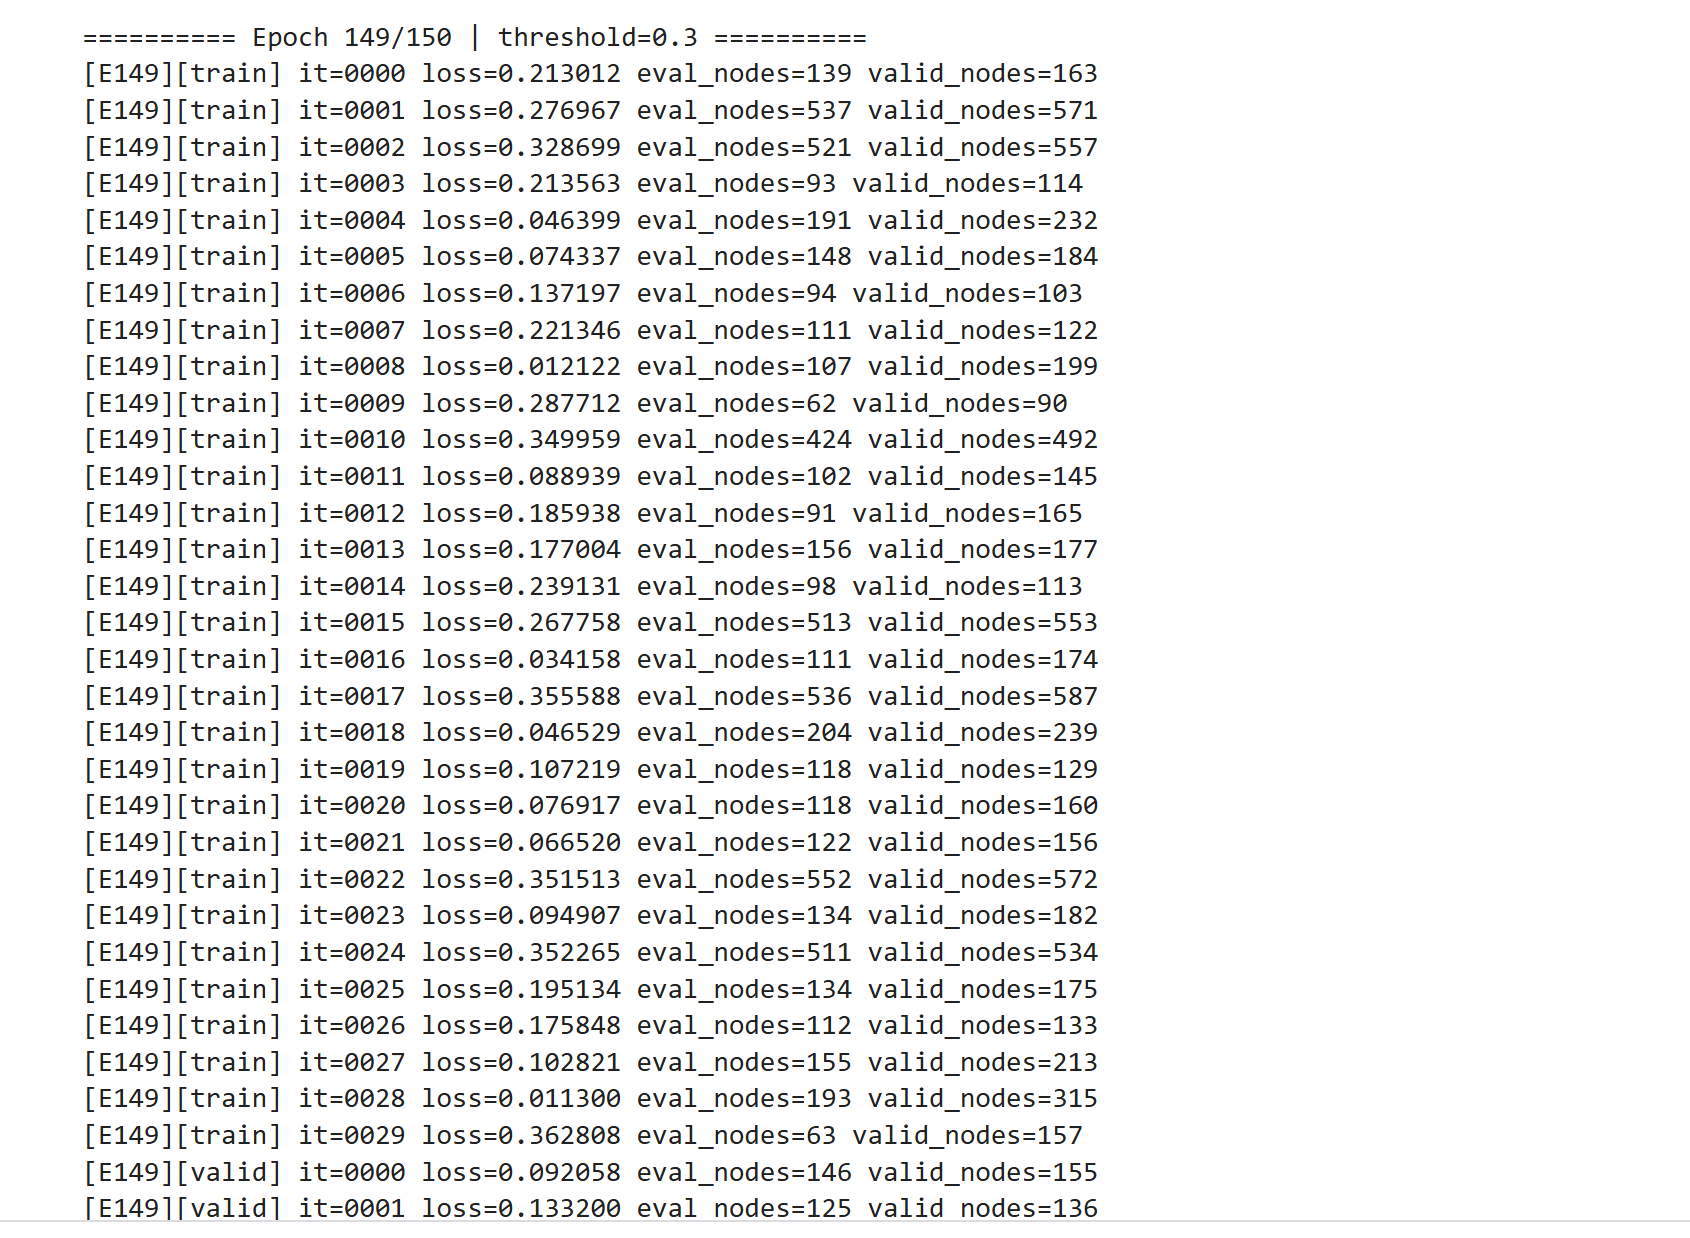
\includegraphics[width=0.8\textwidth]{Contents/MKhang/Epoch149.png}
    \label{fig:model}
\end{figure}
\begin{figure}[H]
    \centering
    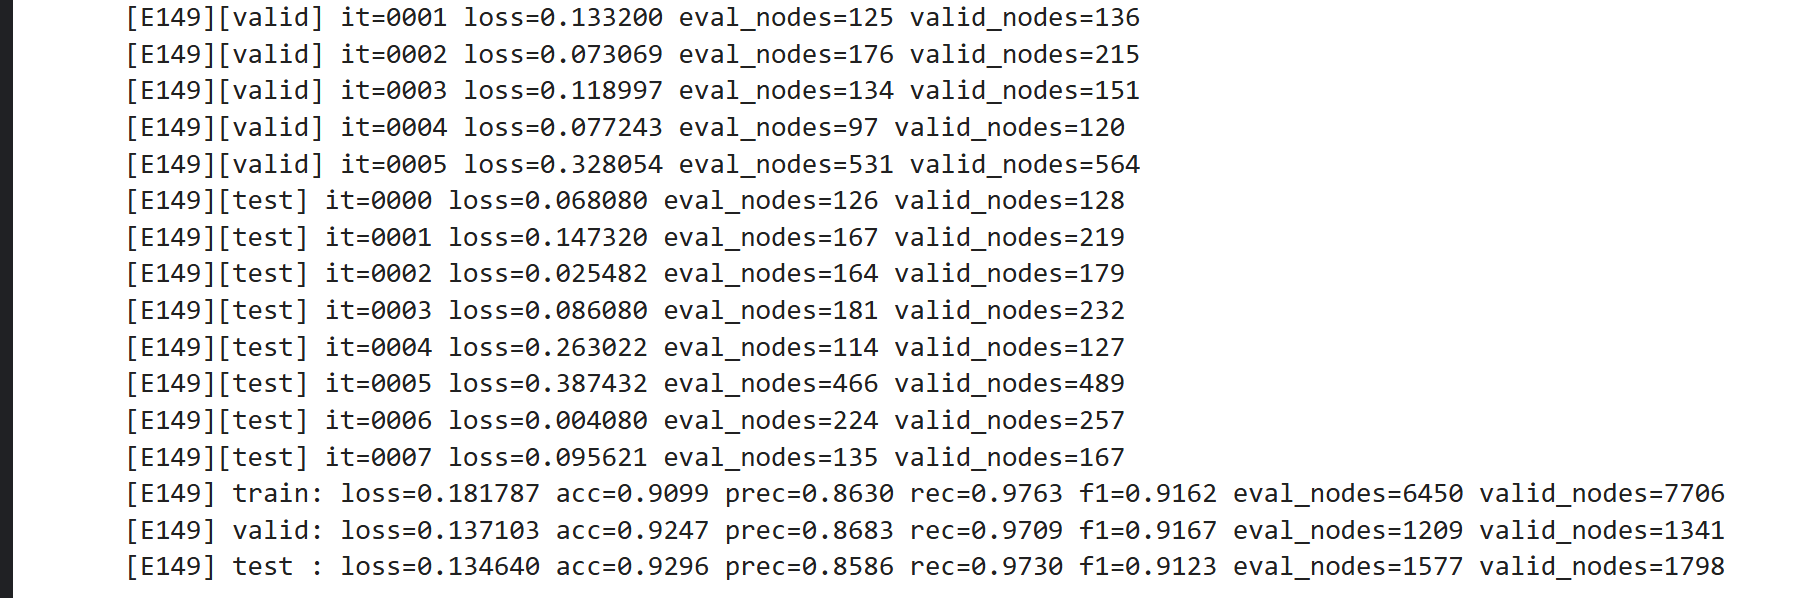
\includegraphics[width=0.8\textwidth]{Contents/MKhang/Epoch149(1).png}
    \caption{Kết quả của Epoch 149}
    \label{fig:model}
\end{figure}

\begin{figure}[H]
    \centering
    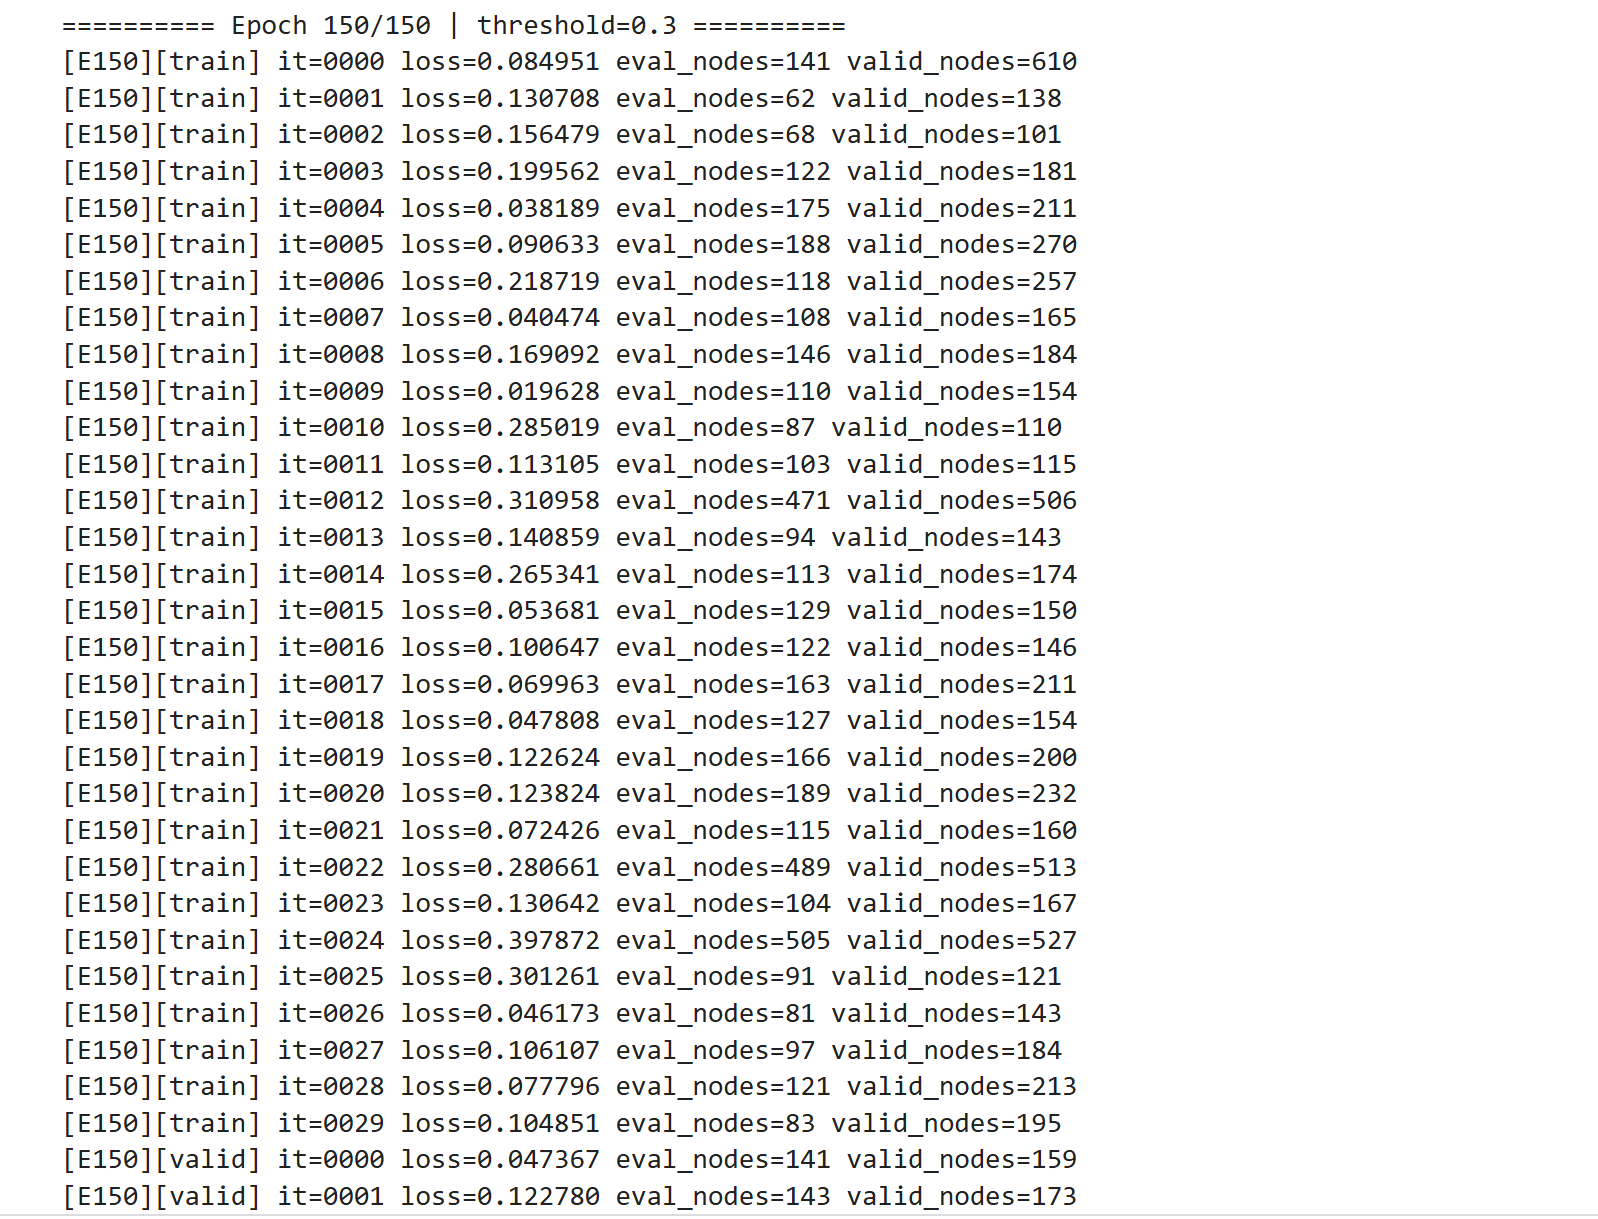
\includegraphics[width=0.8\textwidth]{Contents/MKhang/Epoch150.png}
    \label{fig:model}
\end{figure}
\begin{figure}[H]
    \centering
    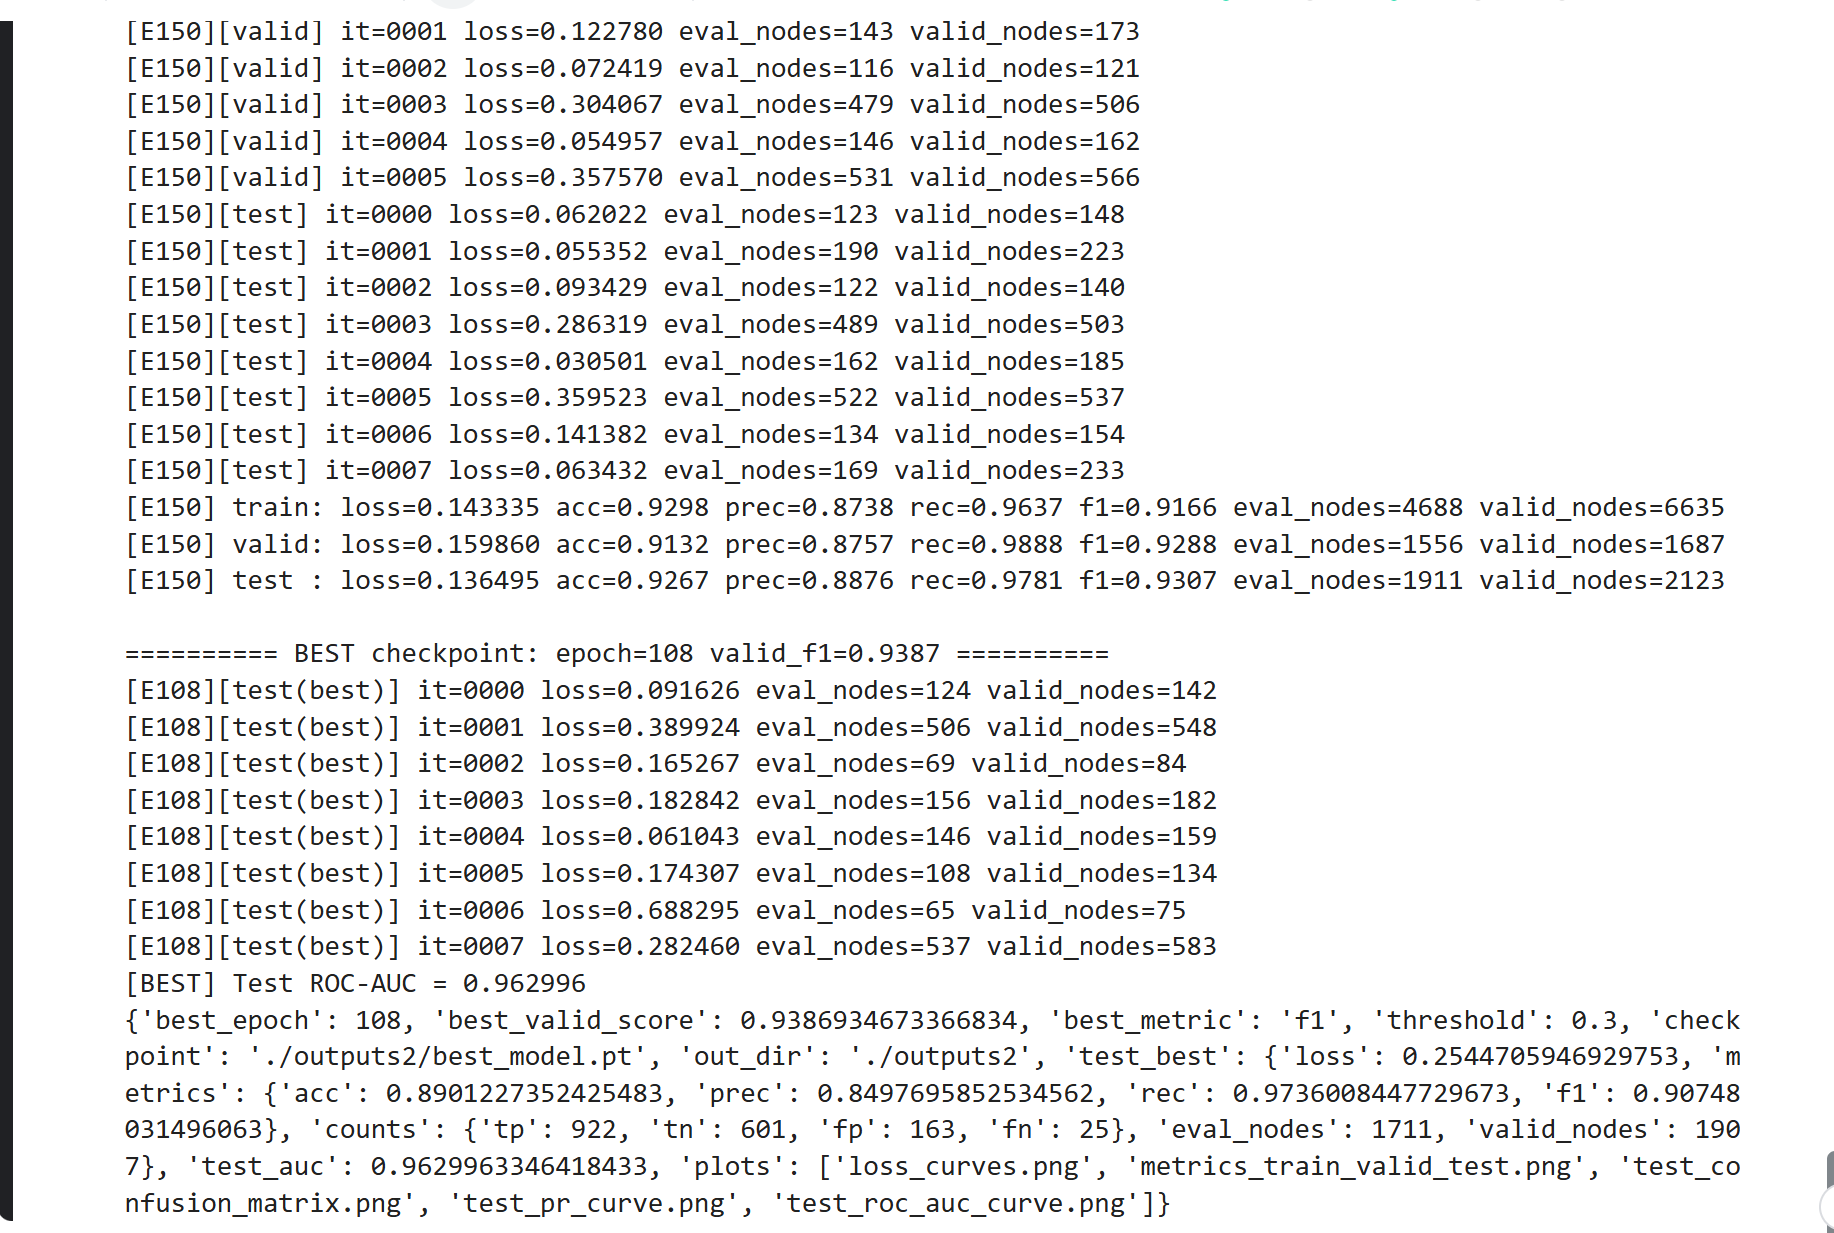
\includegraphics[width=0.8\textwidth]{Contents/MKhang/Epoch150(1).png}
    \caption{Kết quả của Epoch 150}
    \label{fig:model}
\end{figure}
Nhìn chung, có thể quan sát thấy hàm loss giảm dần từ epoch 149 đến epoch 150. Precision duy trì ở mức trên 85\% và Recall ổn định trên 95\% xuyên suốt các epoch trên cả ba tập dữ liệu train, validation và test.

Eval nodes là tổng số node được mô hình dự đoán sau khi áp dụng bước chọn lọc
dựa trên mức độ tương quan mạnh nhất. Valid nodes là tập hợp bao gồm toàn bộ node trong cluster cùng với các eval nodes.

Các chỉ số eval\_nodes, valid\_nodes, TP, FP, TN và FN tại mỗi epoch
được tính bằng cách cộng dồn kết quả từ tất cả các batch trong epoch đó.

\begin{figure}[H]
    \centering
    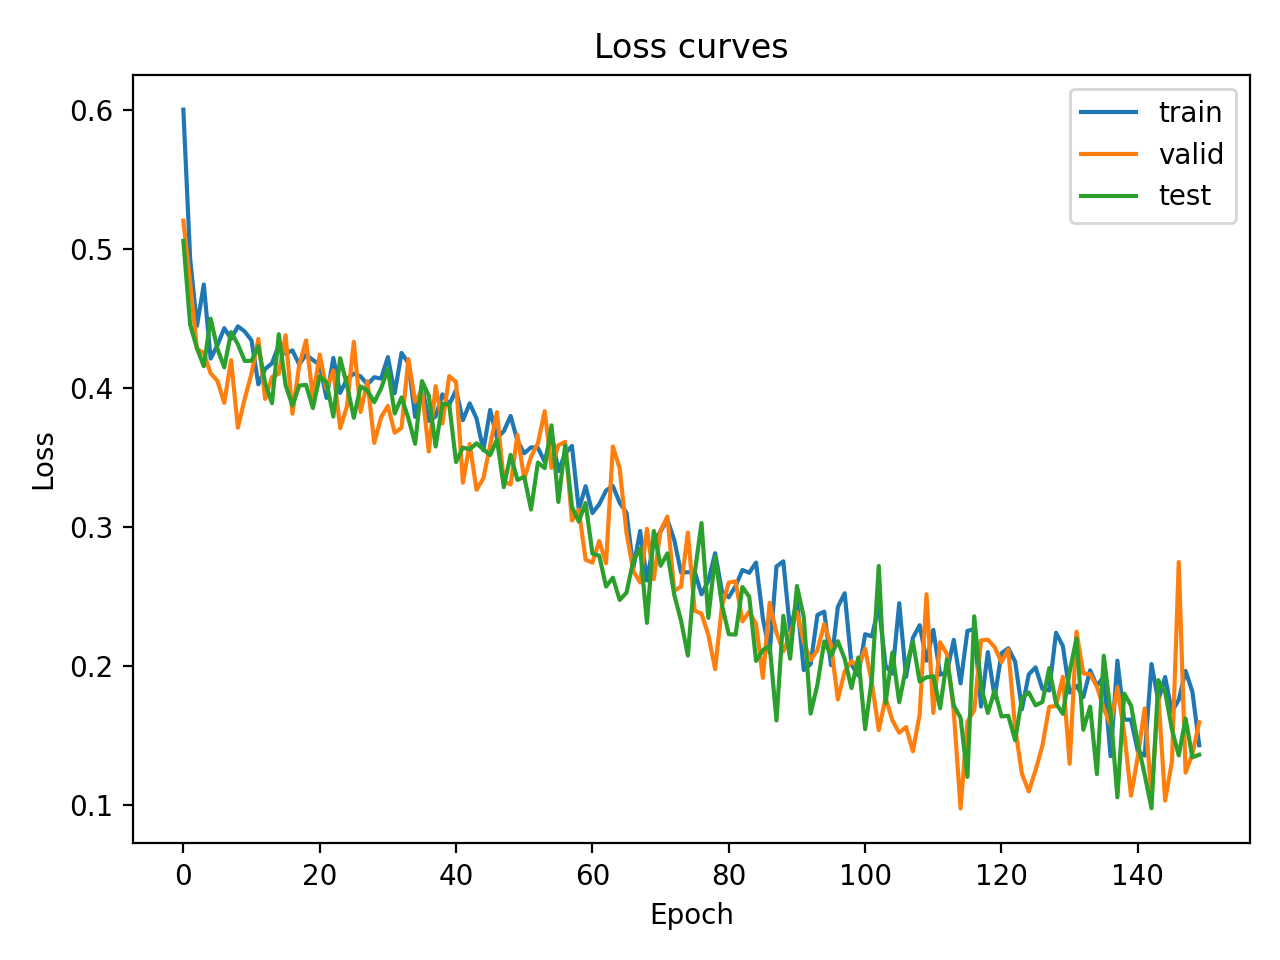
\includegraphics[width=0.8\textwidth]{Contents/MKhang/loss_curves.png}
    \label{fig:loss_curves}

    \caption{Hàm loss qua các epoch}
\end{figure}
Hình trên minh họa diễn biến hàm mất mát trên tập train, validation và test
trong suốt quá trình huấn luyện. Có thể quan sát thấy rằng loss giảm dần và ổn định theo số
epoch, cho thấy mô hình hội tụ tốt và không xuất hiện hiện tượng overfitting nghiêm trọng.
Đường loss của ba tập có xu hướng bám sát nhau, phản ánh khả năng tổng quát hóa tốt của mô
hình đối với dữ liệu chưa từng thấy.

\begin{figure}[H]
    \centering
    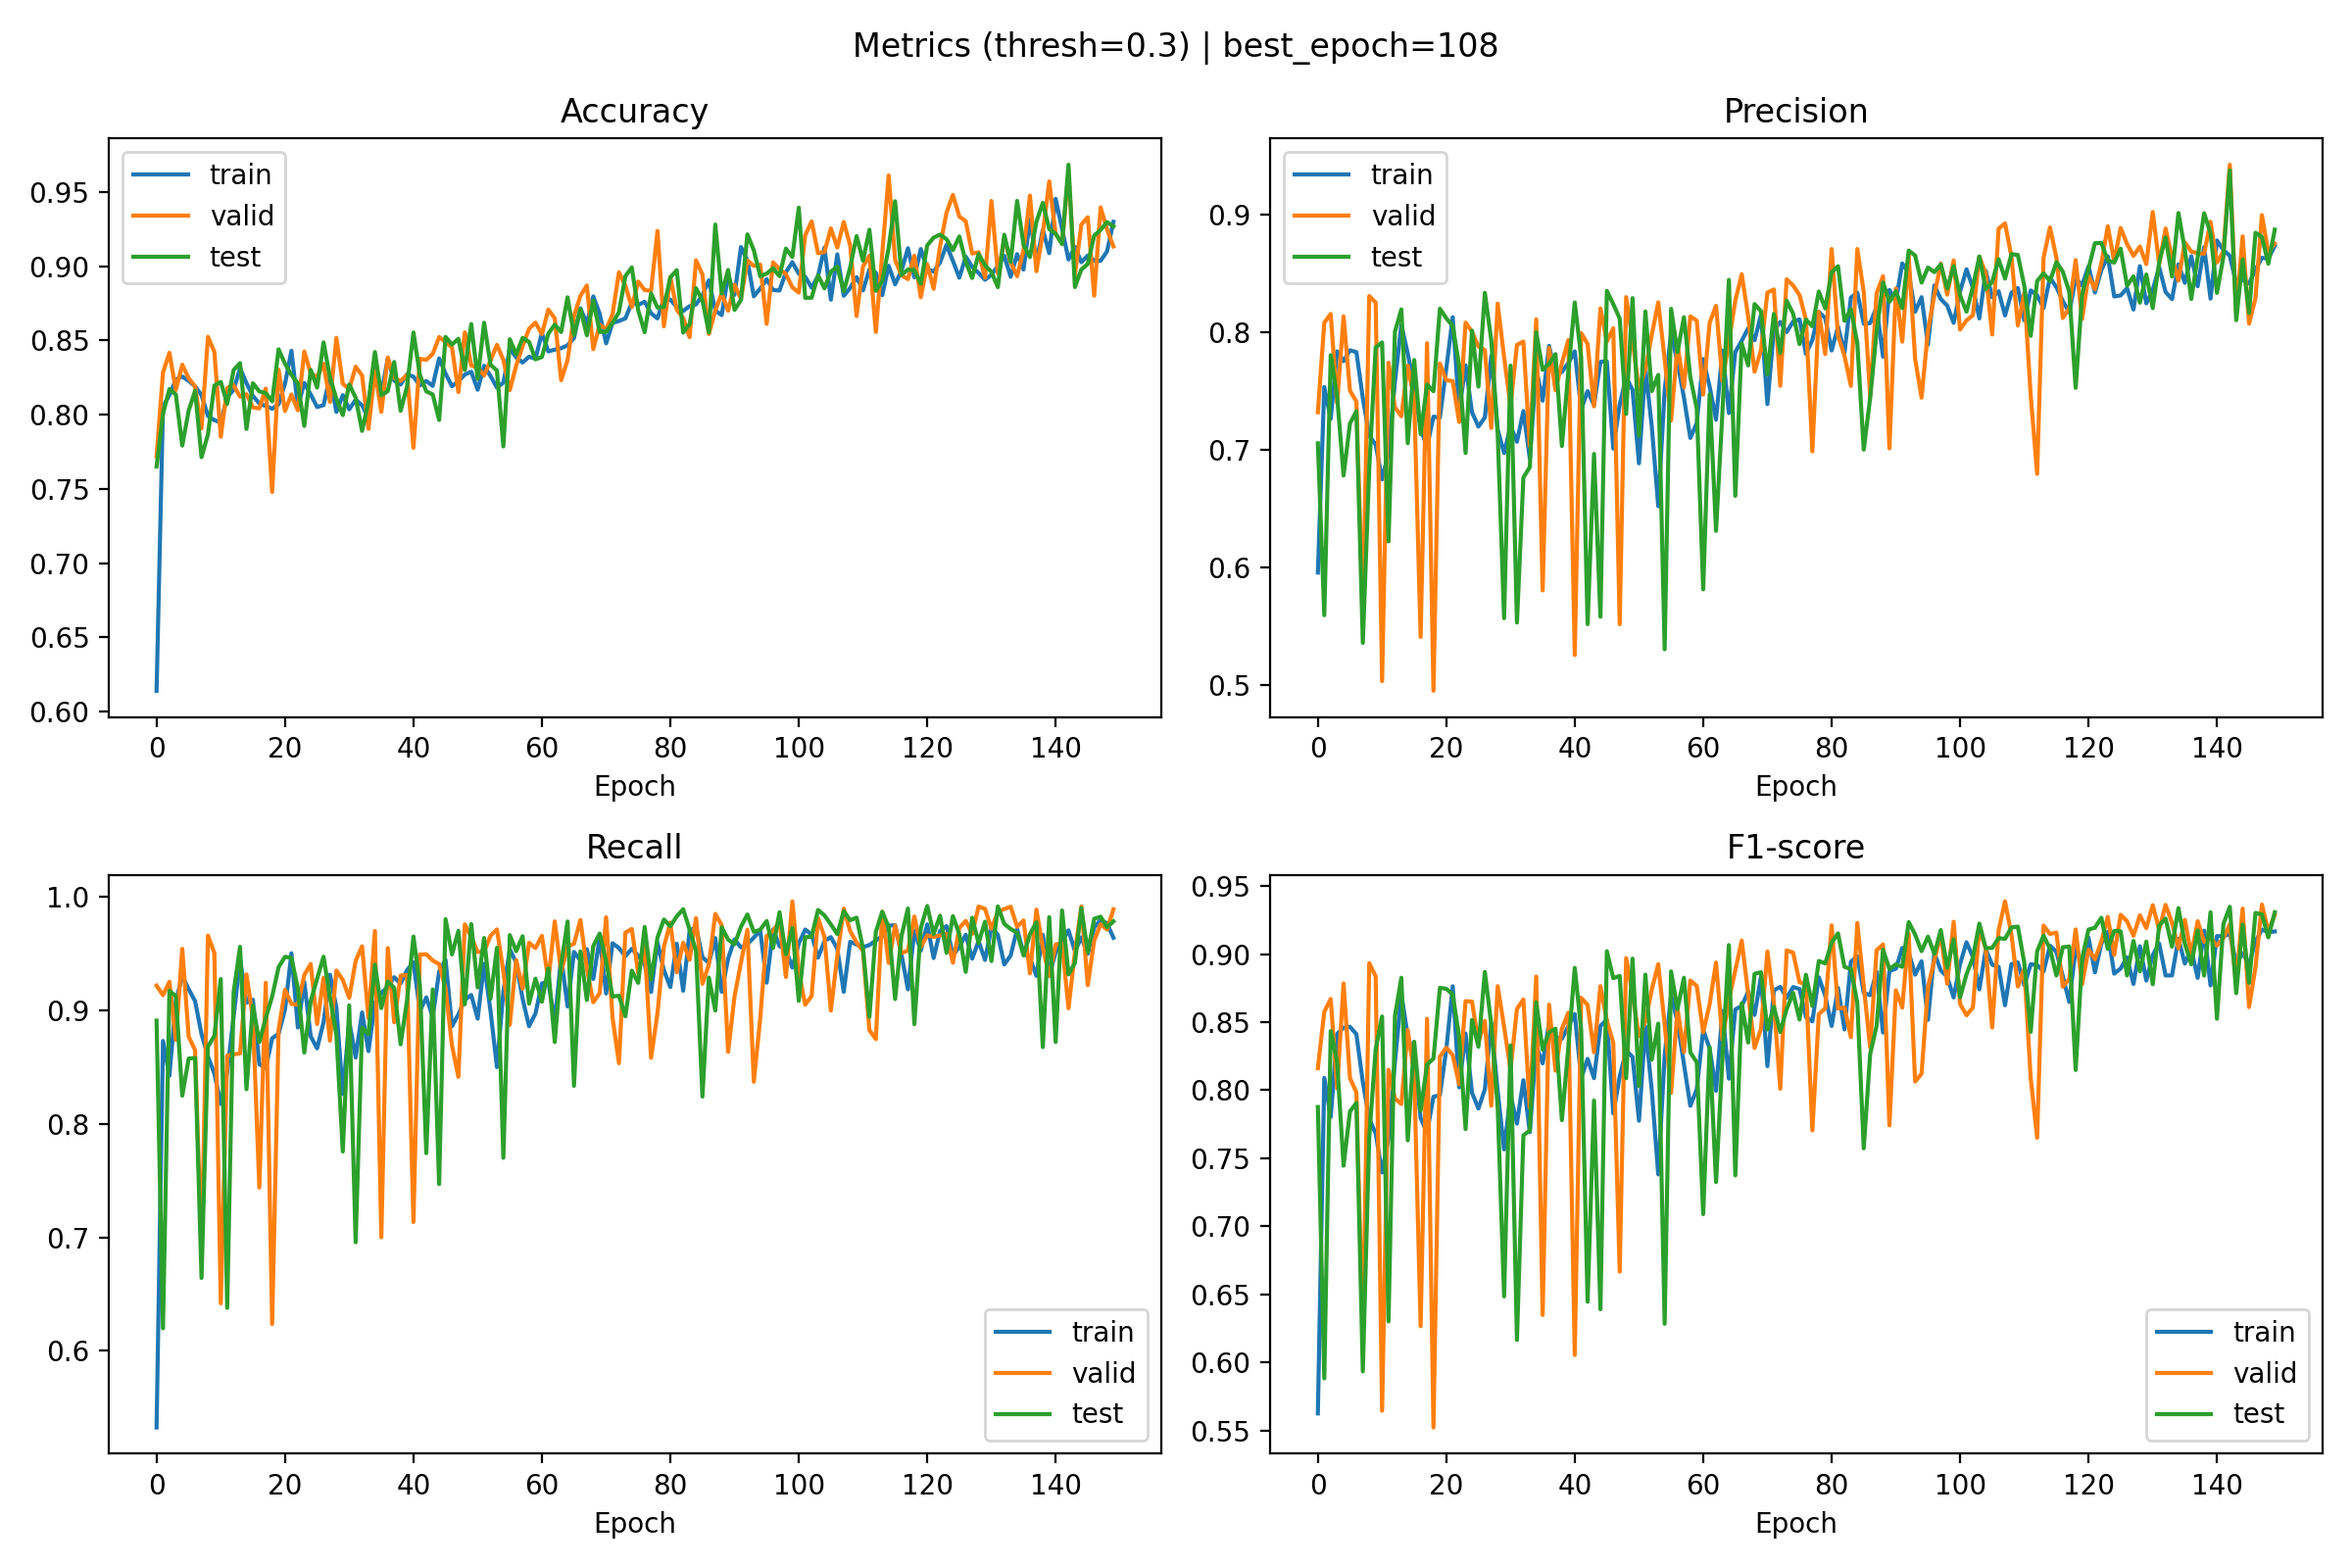
\includegraphics[width=0.8\textwidth]{Contents/MKhang/metrics_train_valid_test.png}
    \label{fig:metrics_train_valid_test}

    \caption{Accuracy, Precision, Recall, F1-score trên train, valid, test qua các epoch}
\end{figure}

Bên cạnh đó, có thể thấy rằng hình trên trình bày sự thay đổi của các chỉ số accuracy,
precision, recall và F1-score theo epoch. Các chỉ số này tăng dần và đạt trạng thái ổn định
sau một số epoch đầu, cho thấy mô hình dần học được các quy luật không gian--thời gian quan
trọng của dữ liệu giao thông.

Dựa trên F1-score của tập validation, checkpoint tốt nhất được lựa chọn tại epoch 108,
và mô hình tại epoch này được sử dụng để đánh giá cuối cùng trên tập test.

\subsection{Đánh giá định lượng trên tập kiểm tra}

Bảng dưới đây tổng hợp các chỉ số đánh giá chính trên tập test tại checkpoint
tốt nhất. Mô hình đạt F1-score cao, cùng với recall lớn, cho thấy khả năng phát hiện các
trạng thái ùn tắc trong tương lai một cách hiệu quả, trong khi vẫn duy trì mức precision
ổn định.

\begin{table}[H]
\centering
\caption{Kết quả định lượng trên tập test (dự đoán 15 phút sau).}
\label{tab:test_metrics}
\begin{tabular}{lcccc}
\hline
Metric & Accuracy & Precision & Recall & F1-score \\
\hline
Test set & 0.89 & 0.85 & 0.97 & 0.91 \\
\hline
\end{tabular}
\end{table}

Giá trị recall cao cho thấy mô hình ít bỏ sót các trường hợp ùn tắc, điều này đặc biệt quan
trọng trong các ứng dụng hỗ trợ điều hành giao thông, nơi việc phát hiện sớm ùn tắc có ý
nghĩa thực tiễn lớn.

\subsection{Phân tích đường cong PR và ROC}

\begin{figure}[H]
    \centering
    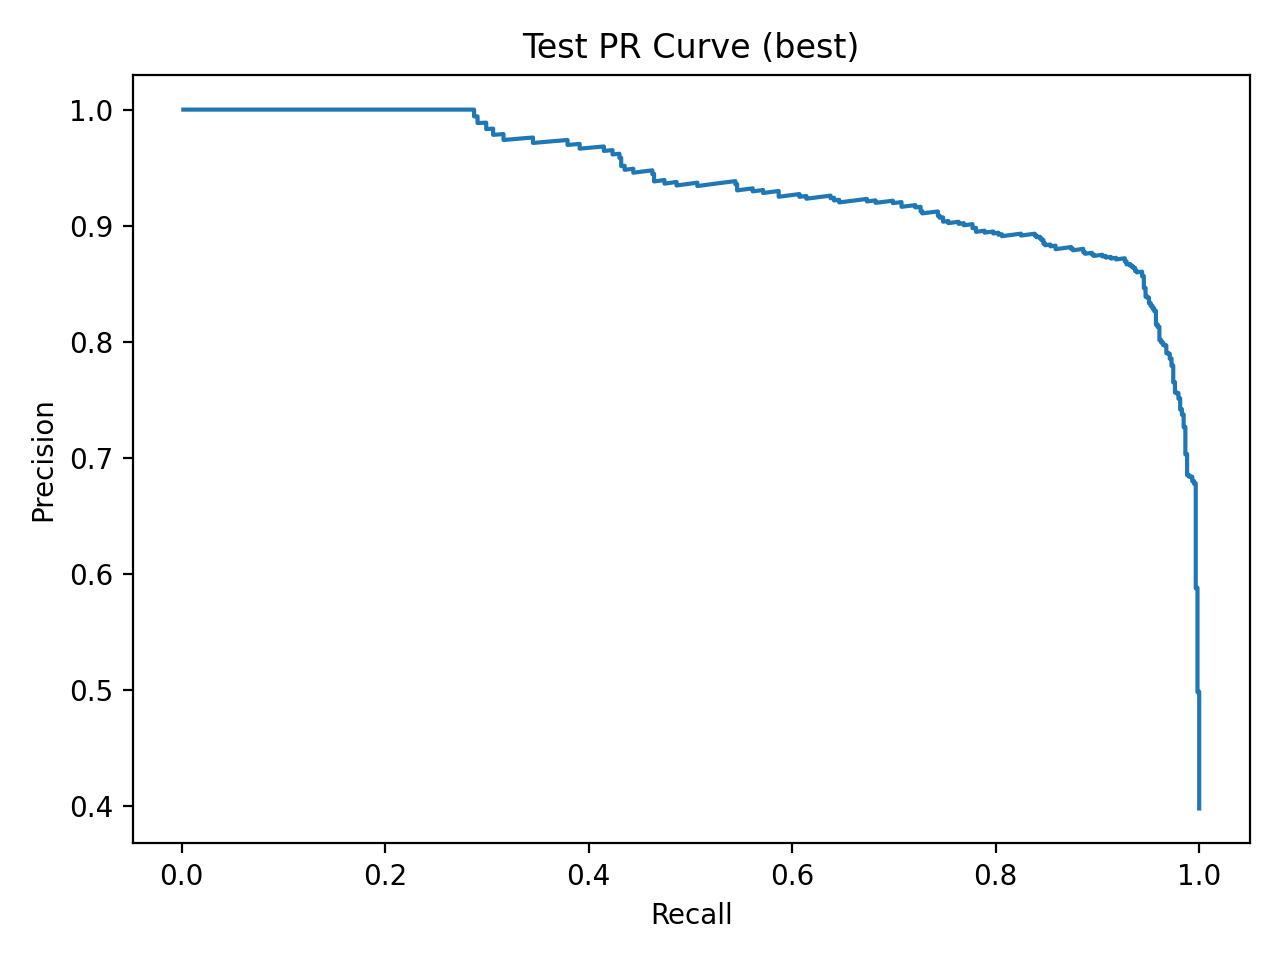
\includegraphics[width=0.8\textwidth]{Contents/MKhang/test_pr_curve.png}

    \caption{Precision-Recall curve}
\end{figure}

Hình trên trình bày đường cong Precision--Recall trên tập test tại checkpoint
tốt nhất. Đường cong cho thấy mô hình duy trì precision cao trong một dải recall rộng, phản
ánh khả năng cân bằng tốt giữa hai tiêu chí này ngay cả khi thay đổi ngưỡng phân loại.

\begin{figure}[H]
    \centering
    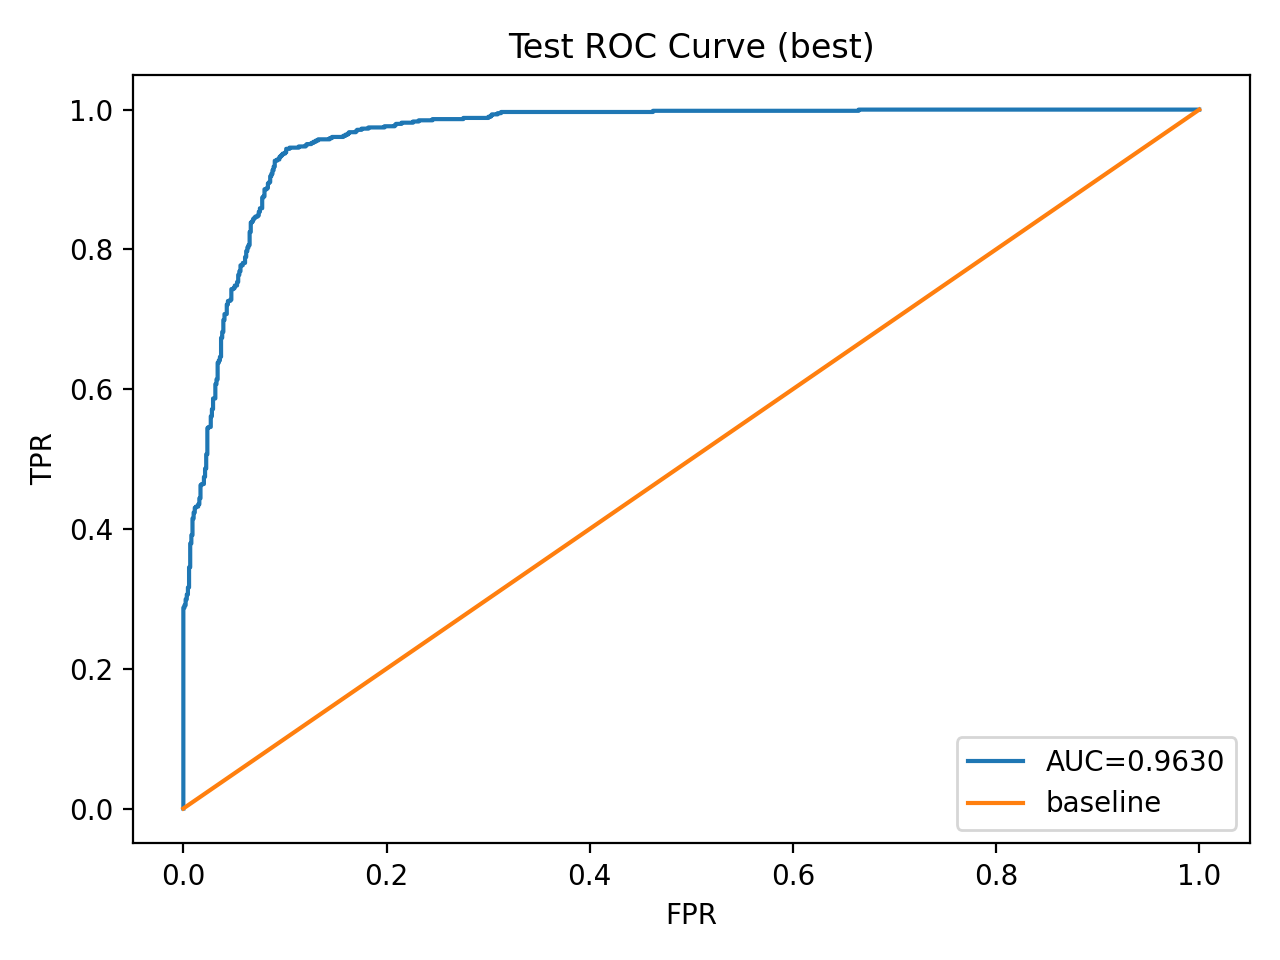
\includegraphics[width=0.8\textwidth]{Contents/MKhang/test_roc_auc_curve.png}

    \caption{ROC,AUC}
\end{figure}
Hình trên minh họa đường cong ROC tương ứng, với diện tích dưới đường cong
(AUC) đạt giá trị cao. Điều này cho thấy mô hình có khả năng phân biệt rõ ràng giữa hai lớp
ùn tắc và không ùn tắc, độc lập với lựa chọn ngưỡng phân loại.

\subsection{Phân tích ma trận nhầm lẫn}
\begin{figure}[H]
    \centering
    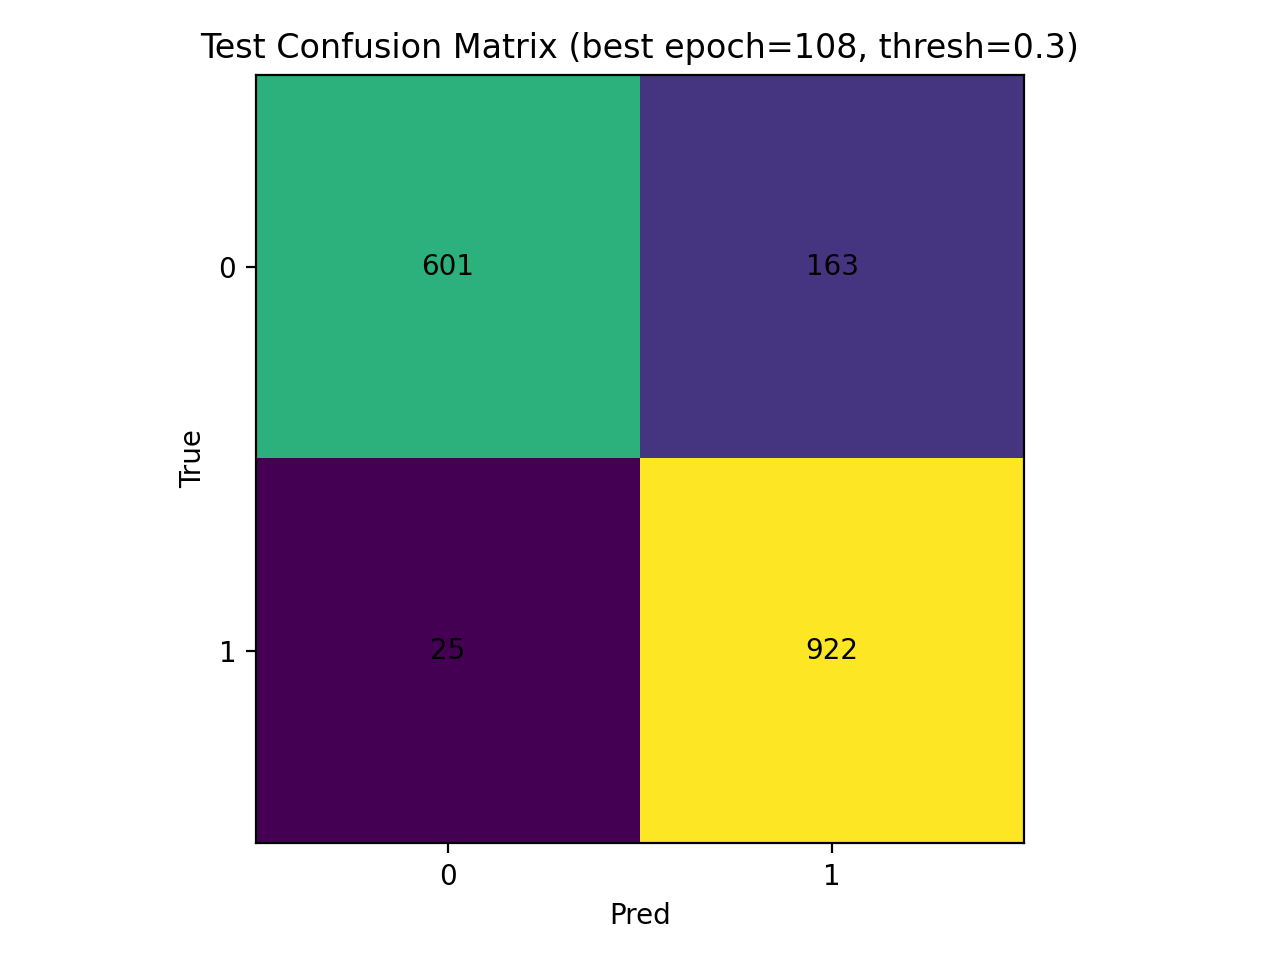
\includegraphics[width=0.8\textwidth]{Contents/MKhang/test_confusion_matrix.png}

    \caption{Ma trận nhầm lẫn}
\end{figure}
Để phân tích chi tiết hơn các dạng sai lệch của mô hình, nhóm sẽ xem xét ma trận nhầm lẫn trên tập test tại checkpoint tốt nhất. Có thể thấy số lượng
false negative là tương đối nhỏ so với true positive, cho thấy mô hình ưu tiên phát hiện
đúng các trạng thái ùn tắc trong tương lai. Ngoài ra, TP và TN khá cao cho thấy khả năng dự đoán tốt của mô hình. Bên cạnh đó, FP ở mức trung bình điều này làm giảm precision của mô hình.
\subsection{Một số số liệu phản ánh khả năng học và dự đoán của mô hình sau 30 phút}

\subsection{Thảo luận}
\label{subsec:discussion}
\begin{figure}[H]
    \centering
    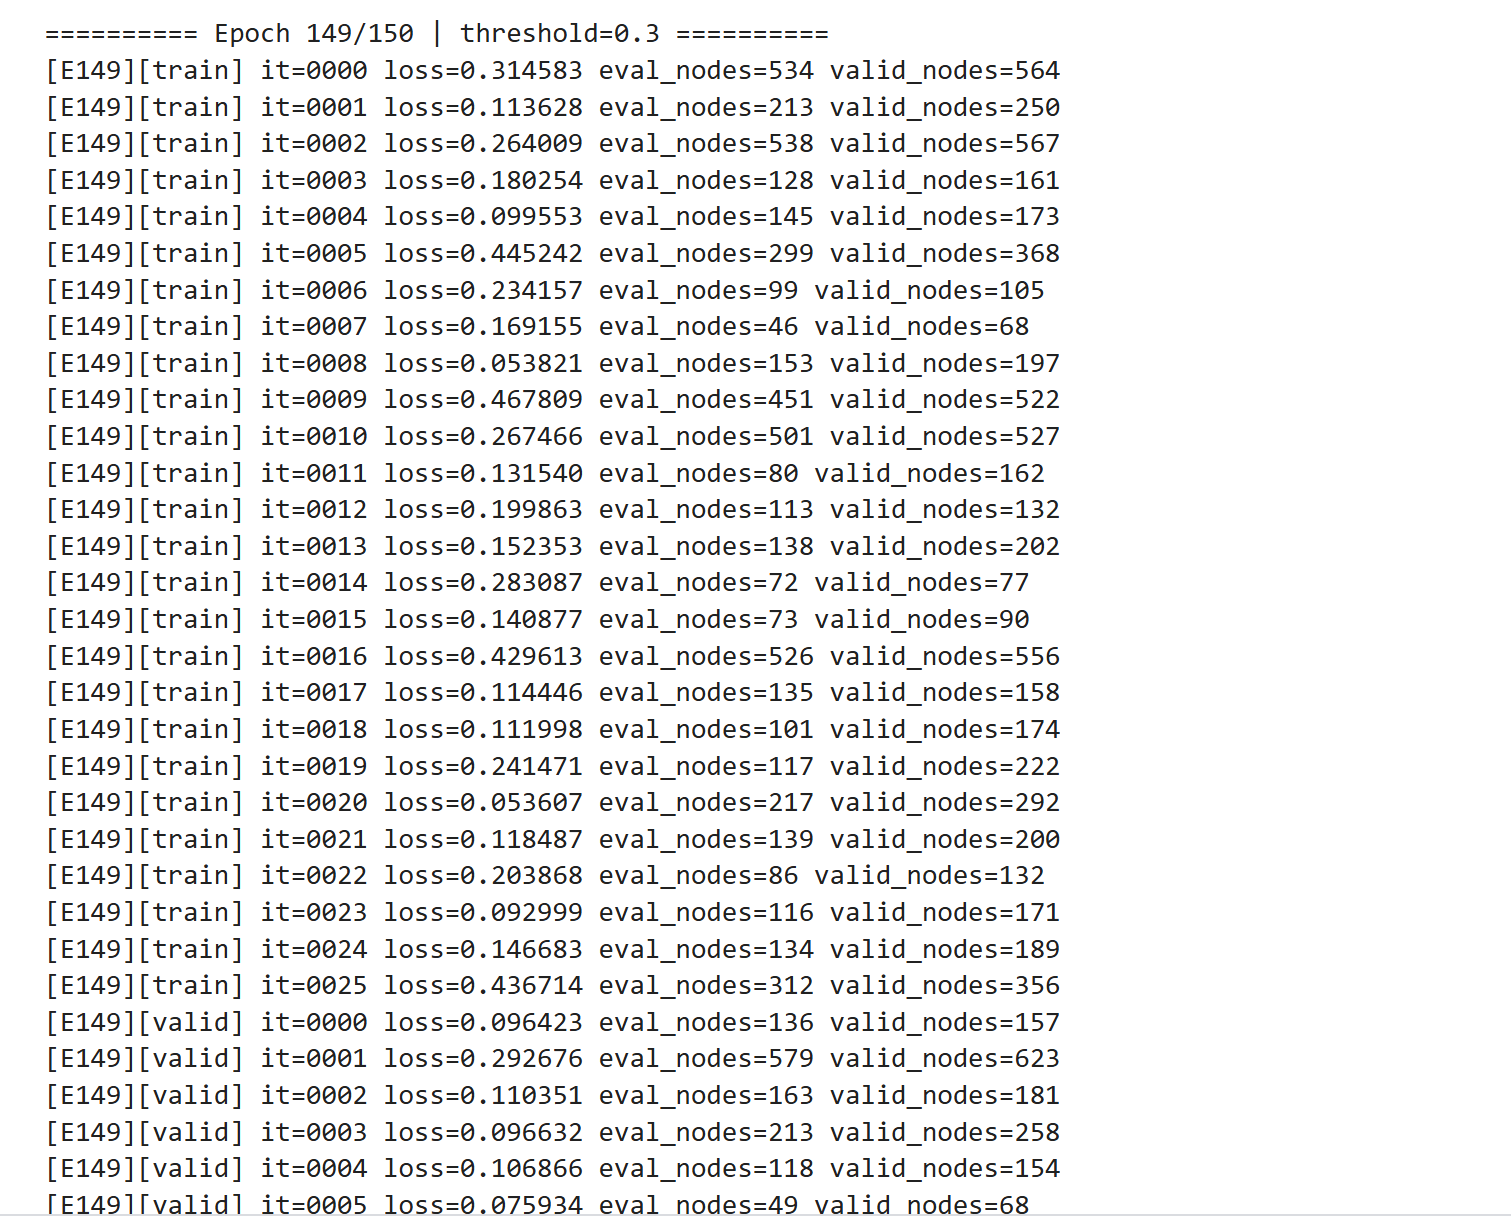
\includegraphics[width=0.8\textwidth]{Contents/MKhang/epoch149_30.png}

\end{figure}
\begin{figure}[H]
    \centering
    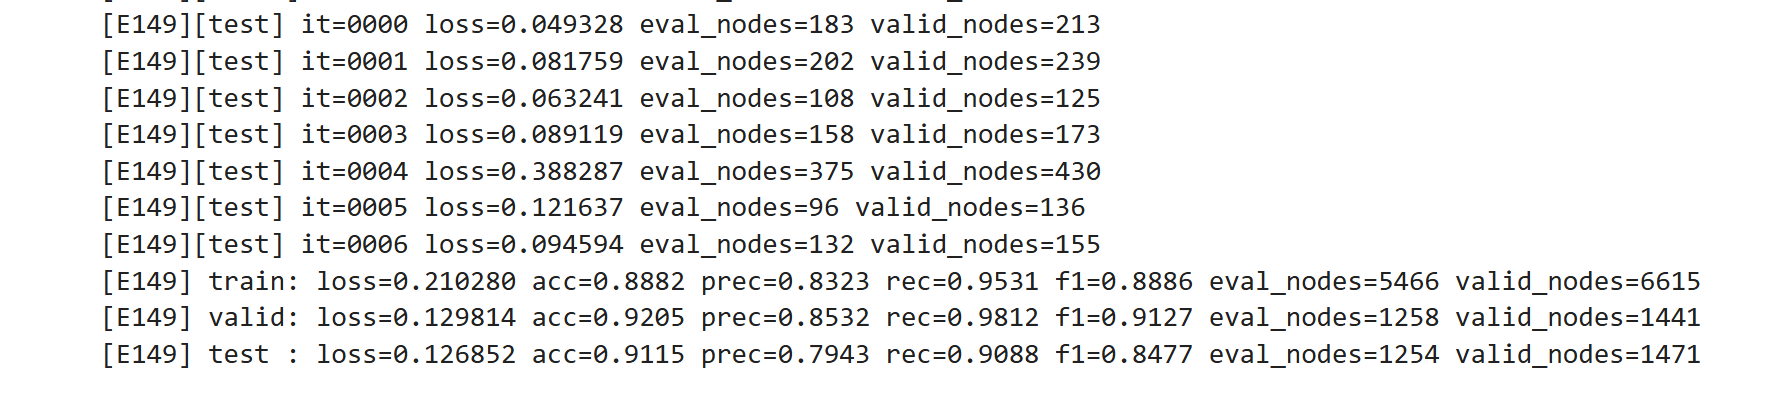
\includegraphics[width=0.8\textwidth]{Contents/MKhang/epoch149_30(1).png}

    \caption{Epoch 149}
\end{figure}
\begin{figure}[H]
    \centering
    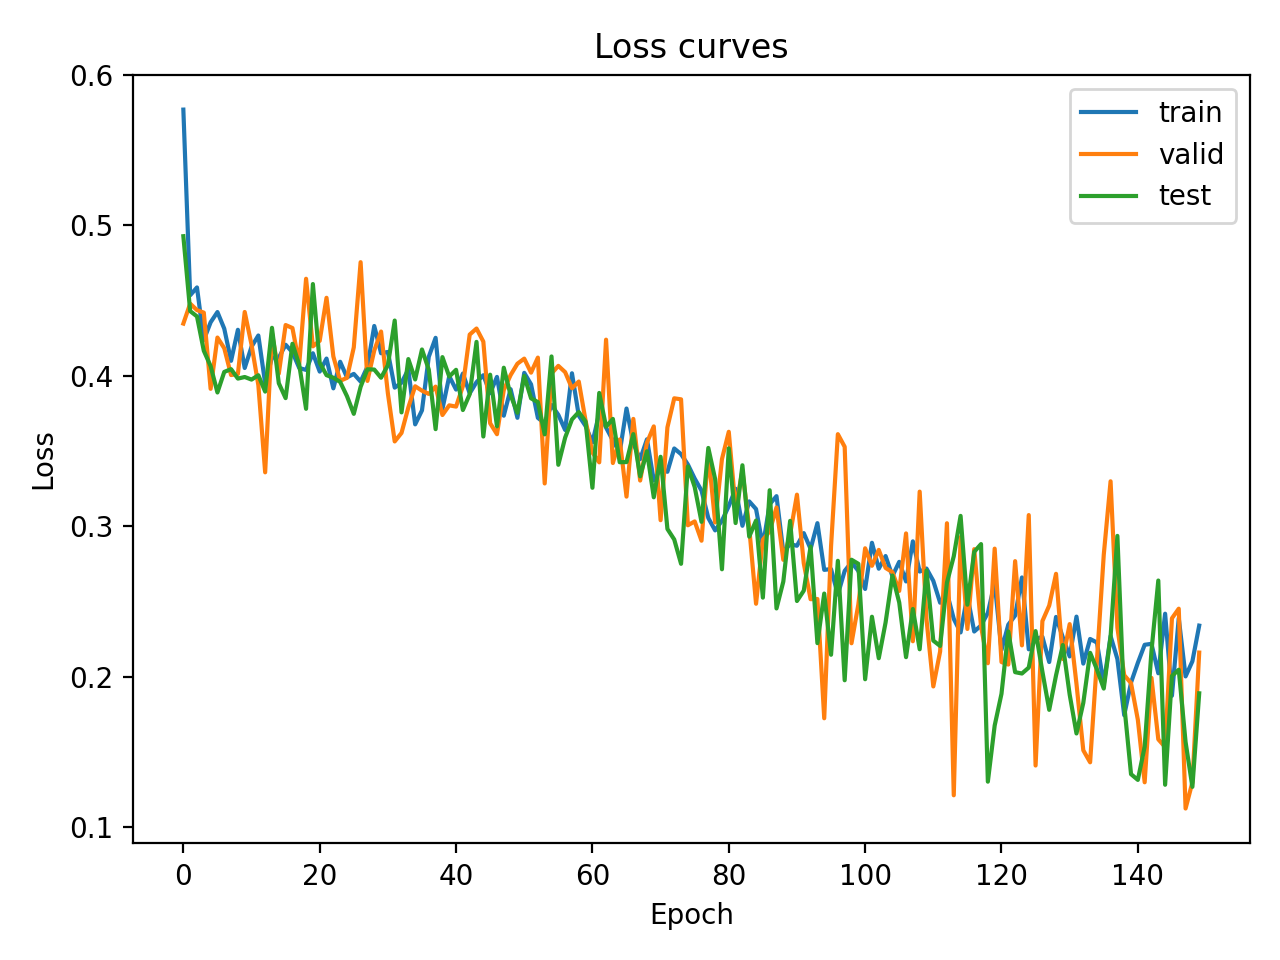
\includegraphics[width=0.8\textwidth]{Contents/MKhang/loss_curves (1).png}

    \caption{Hàm loss qua các epoch}
\end{figure}
\begin{figure}[H]
    \centering
    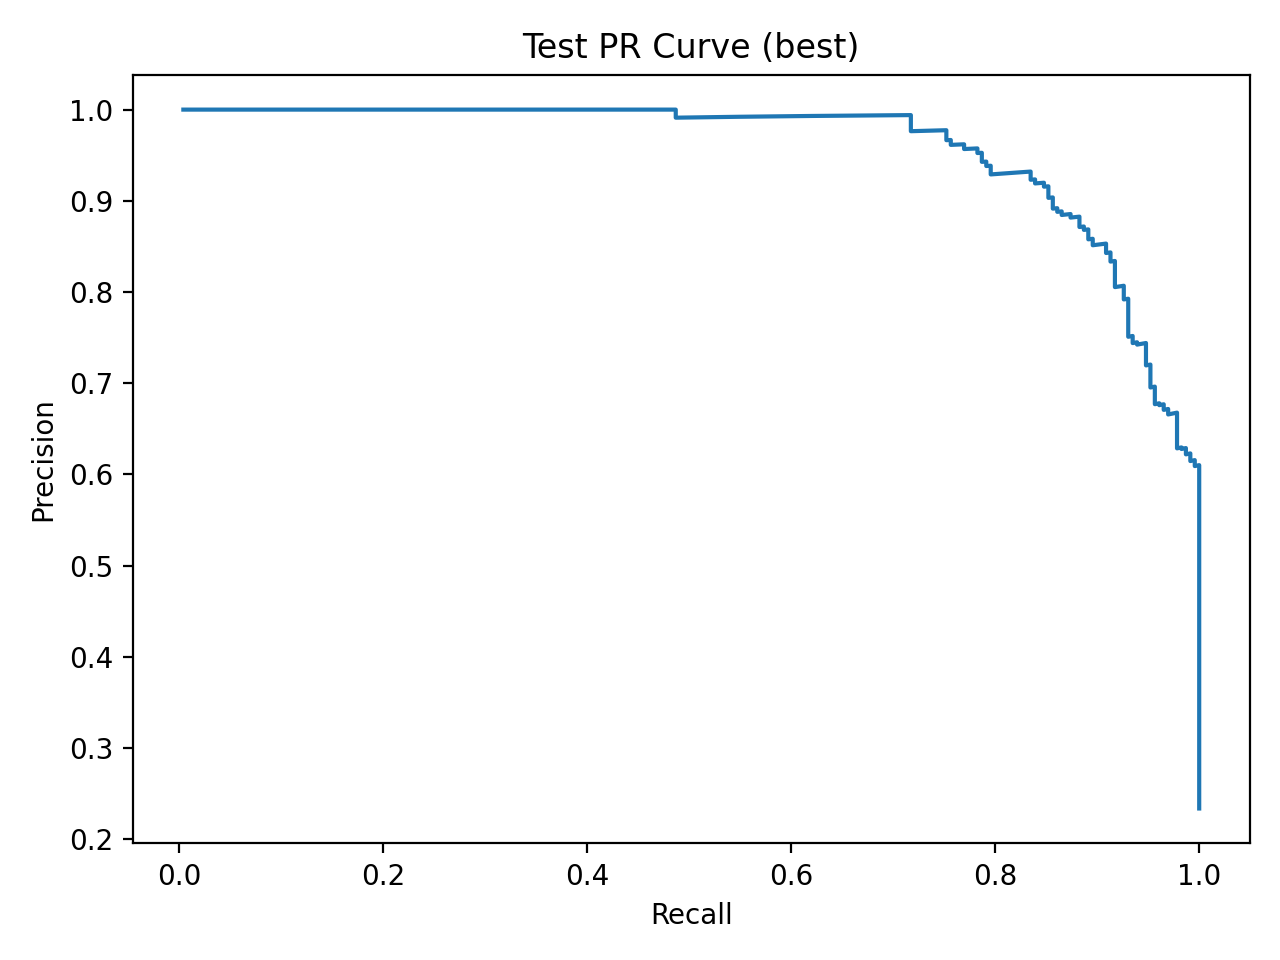
\includegraphics[width=0.8\textwidth]{Contents/MKhang/test_pr_curve (1).png}

    \caption{Precision-Recall curve}
\end{figure}
\begin{figure}[H]
    \centering
    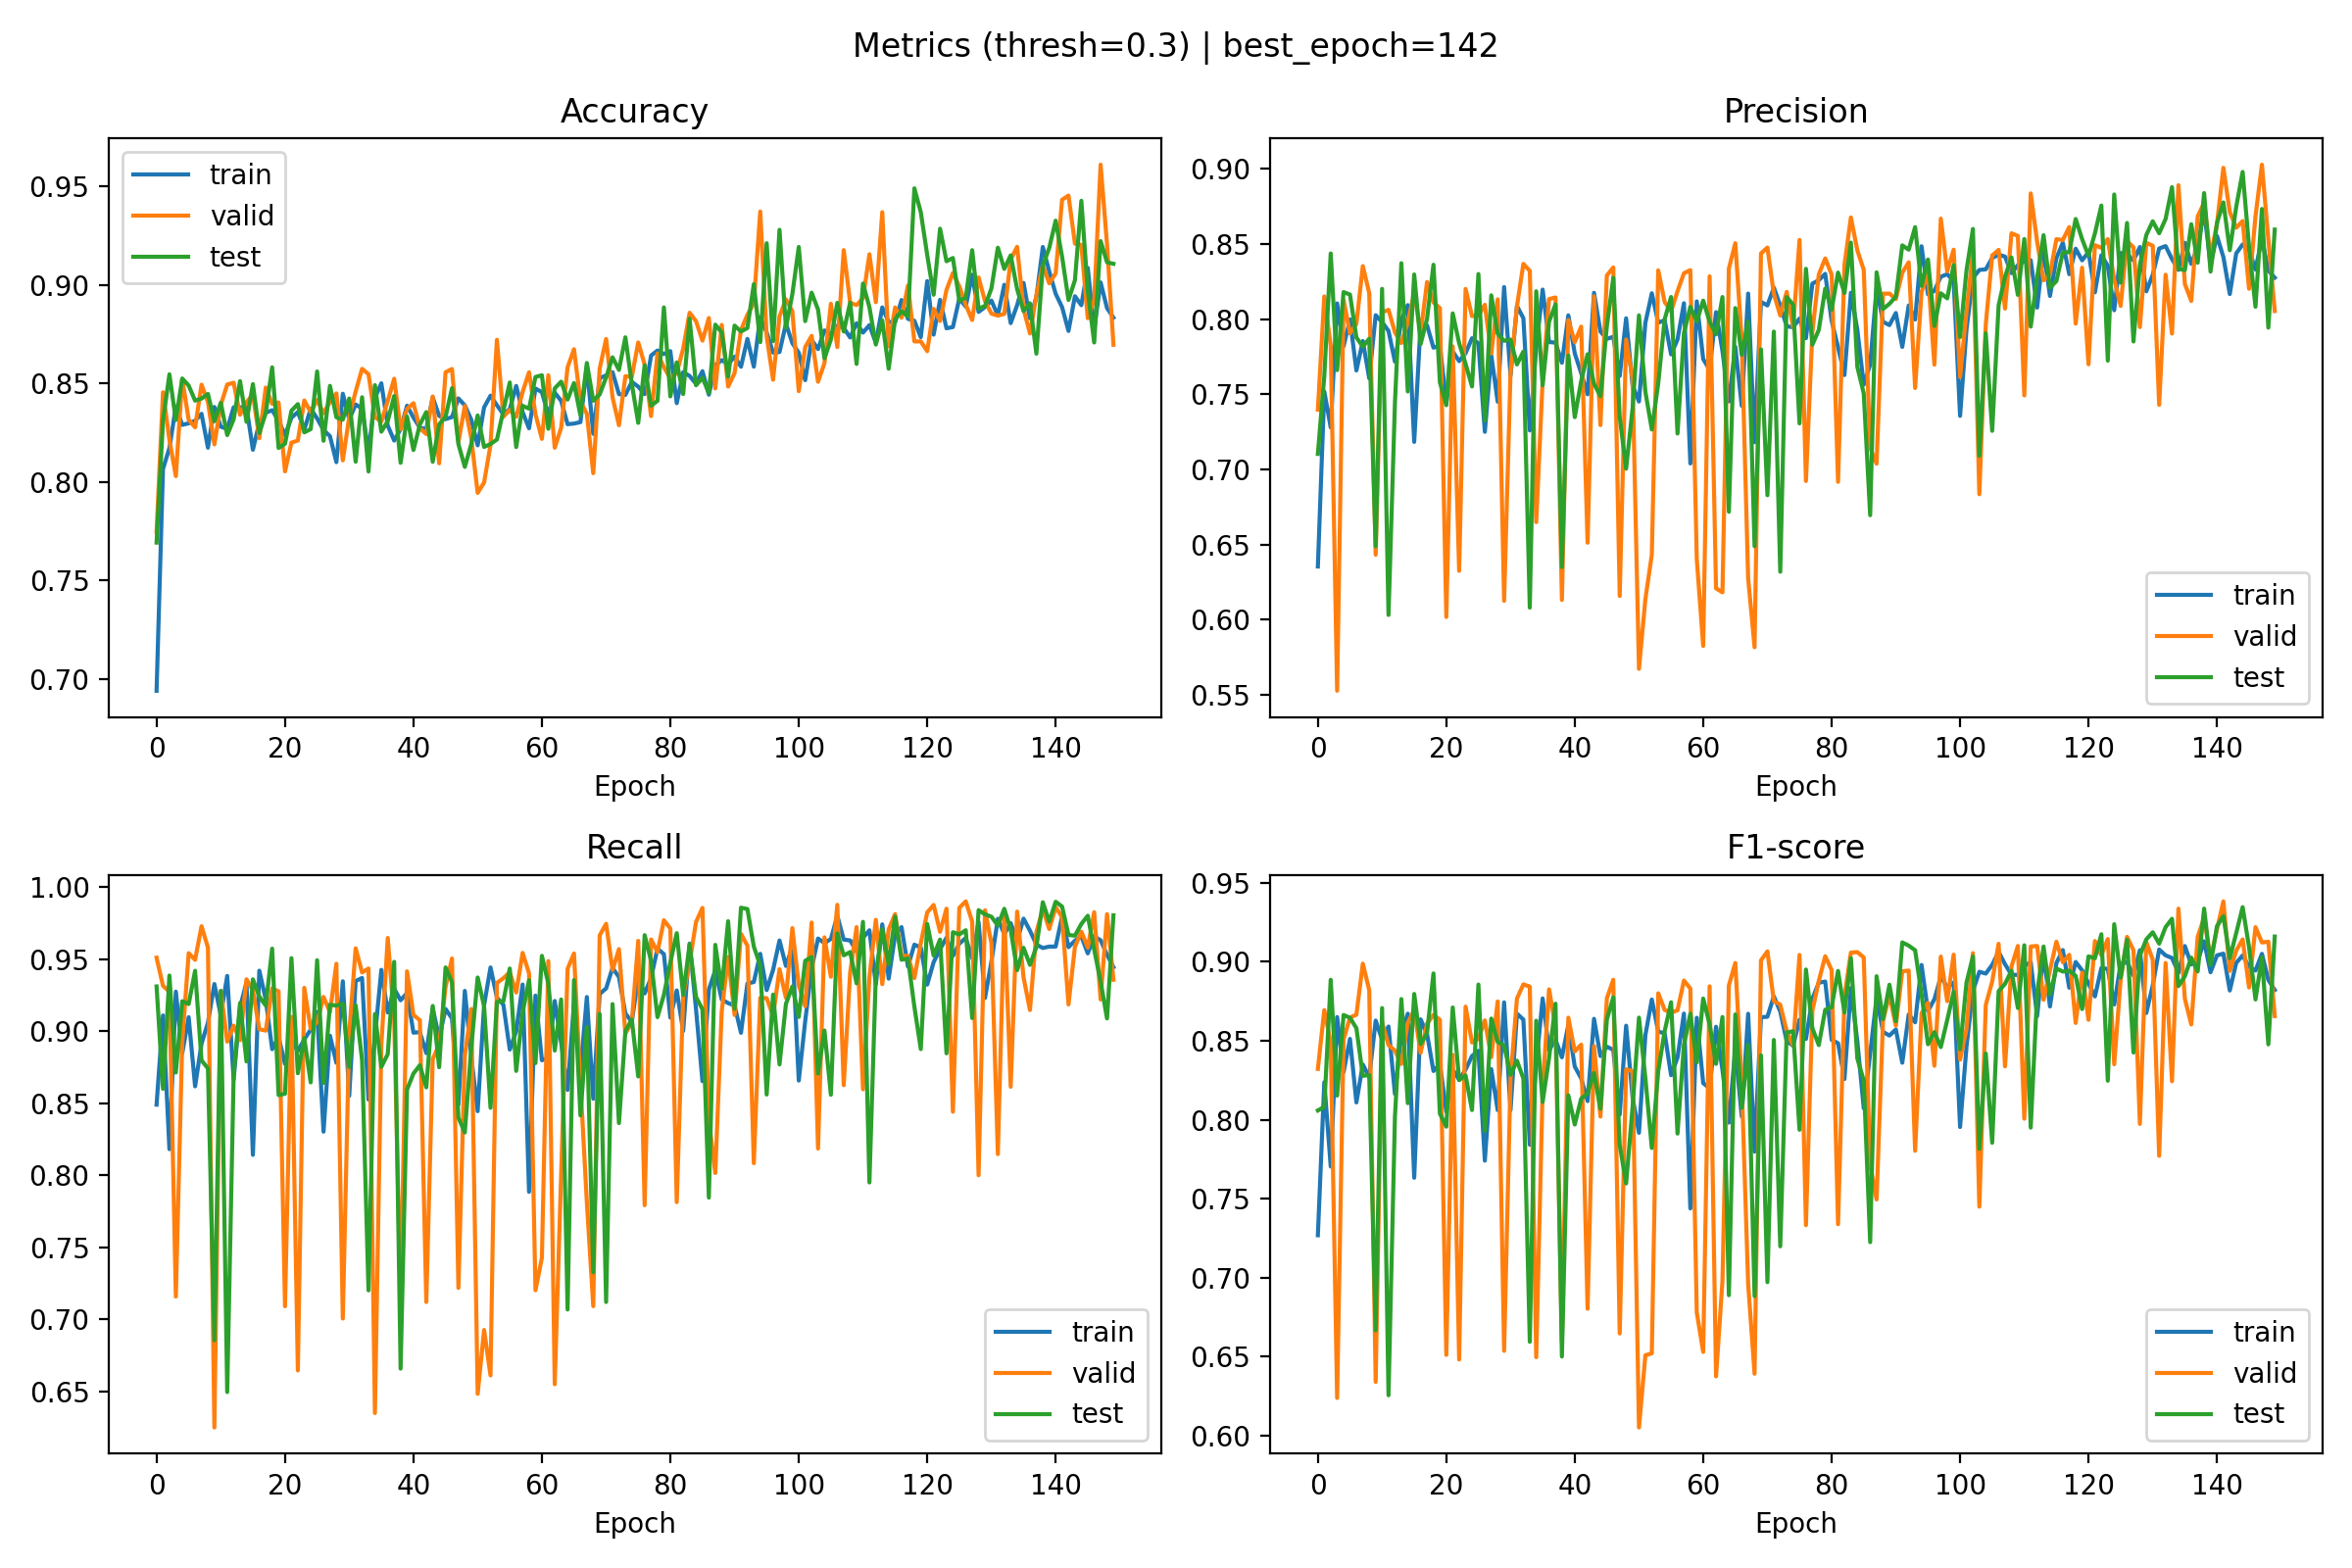
\includegraphics[width=0.8\textwidth]{Contents/MKhang/metrics_train_valid_test (1).png}

    \caption{Precision-Recall curve}
\end{figure}
Ở đây mô hình được nạp và học dữ liệu lại và điều chính để cho đúng với nhãn kẹt hoặc không kẹt 30 phút sau. Nhìn chung mô hình vẫn học được tốt, các hàm loss vẫn giảm đều và số liệu vẫn cho thấy mô hình có khả năng học được tốt

Kết quả thực nghiệm cho thấy mô hình Transformer đề xuất, với việc tích hợp bias vào
attention score và các mã hóa không gian--thời gian, có khả năng dự báo hiệu quả trạng thái
ùn tắc trong tương lai ngắn hạn (15 phút, 30 phút, ...). Sự ổn định của quá trình huấn luyện và các chỉ số
đánh giá cao trên tập test cho thấy mô hình không chỉ học tốt trên dữ liệu huấn luyện mà còn
tổng quát hóa tốt sang dữ liệu chưa từng thấy.
